The Higgs field $\phi$ is a complex scalar field with a potential $V(\phi)$ of the form:
\begin{equation}
    V(\phi) = -\frac{1}{2}\mu^2|\phi|^2 + \frac{1}{4}\lambda|\phi|^4,
\end{equation}
where $\lambda$ and $\mu$ are parameters (ultimately related to the Higgs self-coupling and Higgs mass). The potential has the famous ``mexican hat'' shape, symmetric about rotations in $\phi$, with a non-zero minimum expectation value $\braket{\phi} \neq 0$, as seen in the graph in Fig.~\ref{fig:HiggsPotential}. Initially, the Higgs potential exisits in the unstable state where $\braket{\phi} = 0$, preserving the $\phi$ symmetry. A fluctuation in the Higgs field will minimize the potential as $\phi$ aquires some non-zero vacuum expectation value (VEV) $\braket{0|\phi|0} = v$, and in doing so breaks the rotational symmetry of $\phi$; this is called spontaneous symmetry breaking. It is convenient to now parameterize $\phi$ in terms of two real scalar fields $h$ and $\chi$ and expand about $v$, like:
\begin{equation}
    \phi = \frac{1}{\sqrt{2}}(v+h)e^{i\chi/v},
\end{equation}
and after substituting the fields back into the lagrangian, we emerge with a massive physical higgs boson $h$ and a massles ``Goldstone'' boson $\chi$.

In EWT, the spontaneous symmetry breaking of the Higgs field is embedded in the $\SUtwoW\times\UoneY$ local gauge symmetry, where the Higgs field is now a weak isospin doublet. In a similar way to the above example, the electroweak symmetry is broken, and we are left with a massive Higgs field, and four massles Goldstone bosons. Through chosing a gauge, the Goldstone bosons are ``eaten'' and we are left with the physical gauge bososns of EWT: a massles photon and three massive weak gauge bosons. 

The SM fermions couple to the Higgs field with so-called Yukawa couplings, like $\antispinor{\Plepton}{L}{}\phi\spinor{\Pe}{R}{}$, $\antispinor{\Pquark}{L}{}\phi\spinor{\Pdown}{R}{}$, and $\antispinor{\Pquark}{L}{}\tilde{\phi}\spinor{\Pup}{R}{}$ which form weak isospin singlets. After spontaneous symmetry breaking of the Higgs field, the fermions aquire masses in a similar way to the gauge bosons, while the absence of any right-handed neutrinos in the SM prevents them from coupling to the Higgs field and leaves them massless.

\begin{figure}[H]
    \centering
    {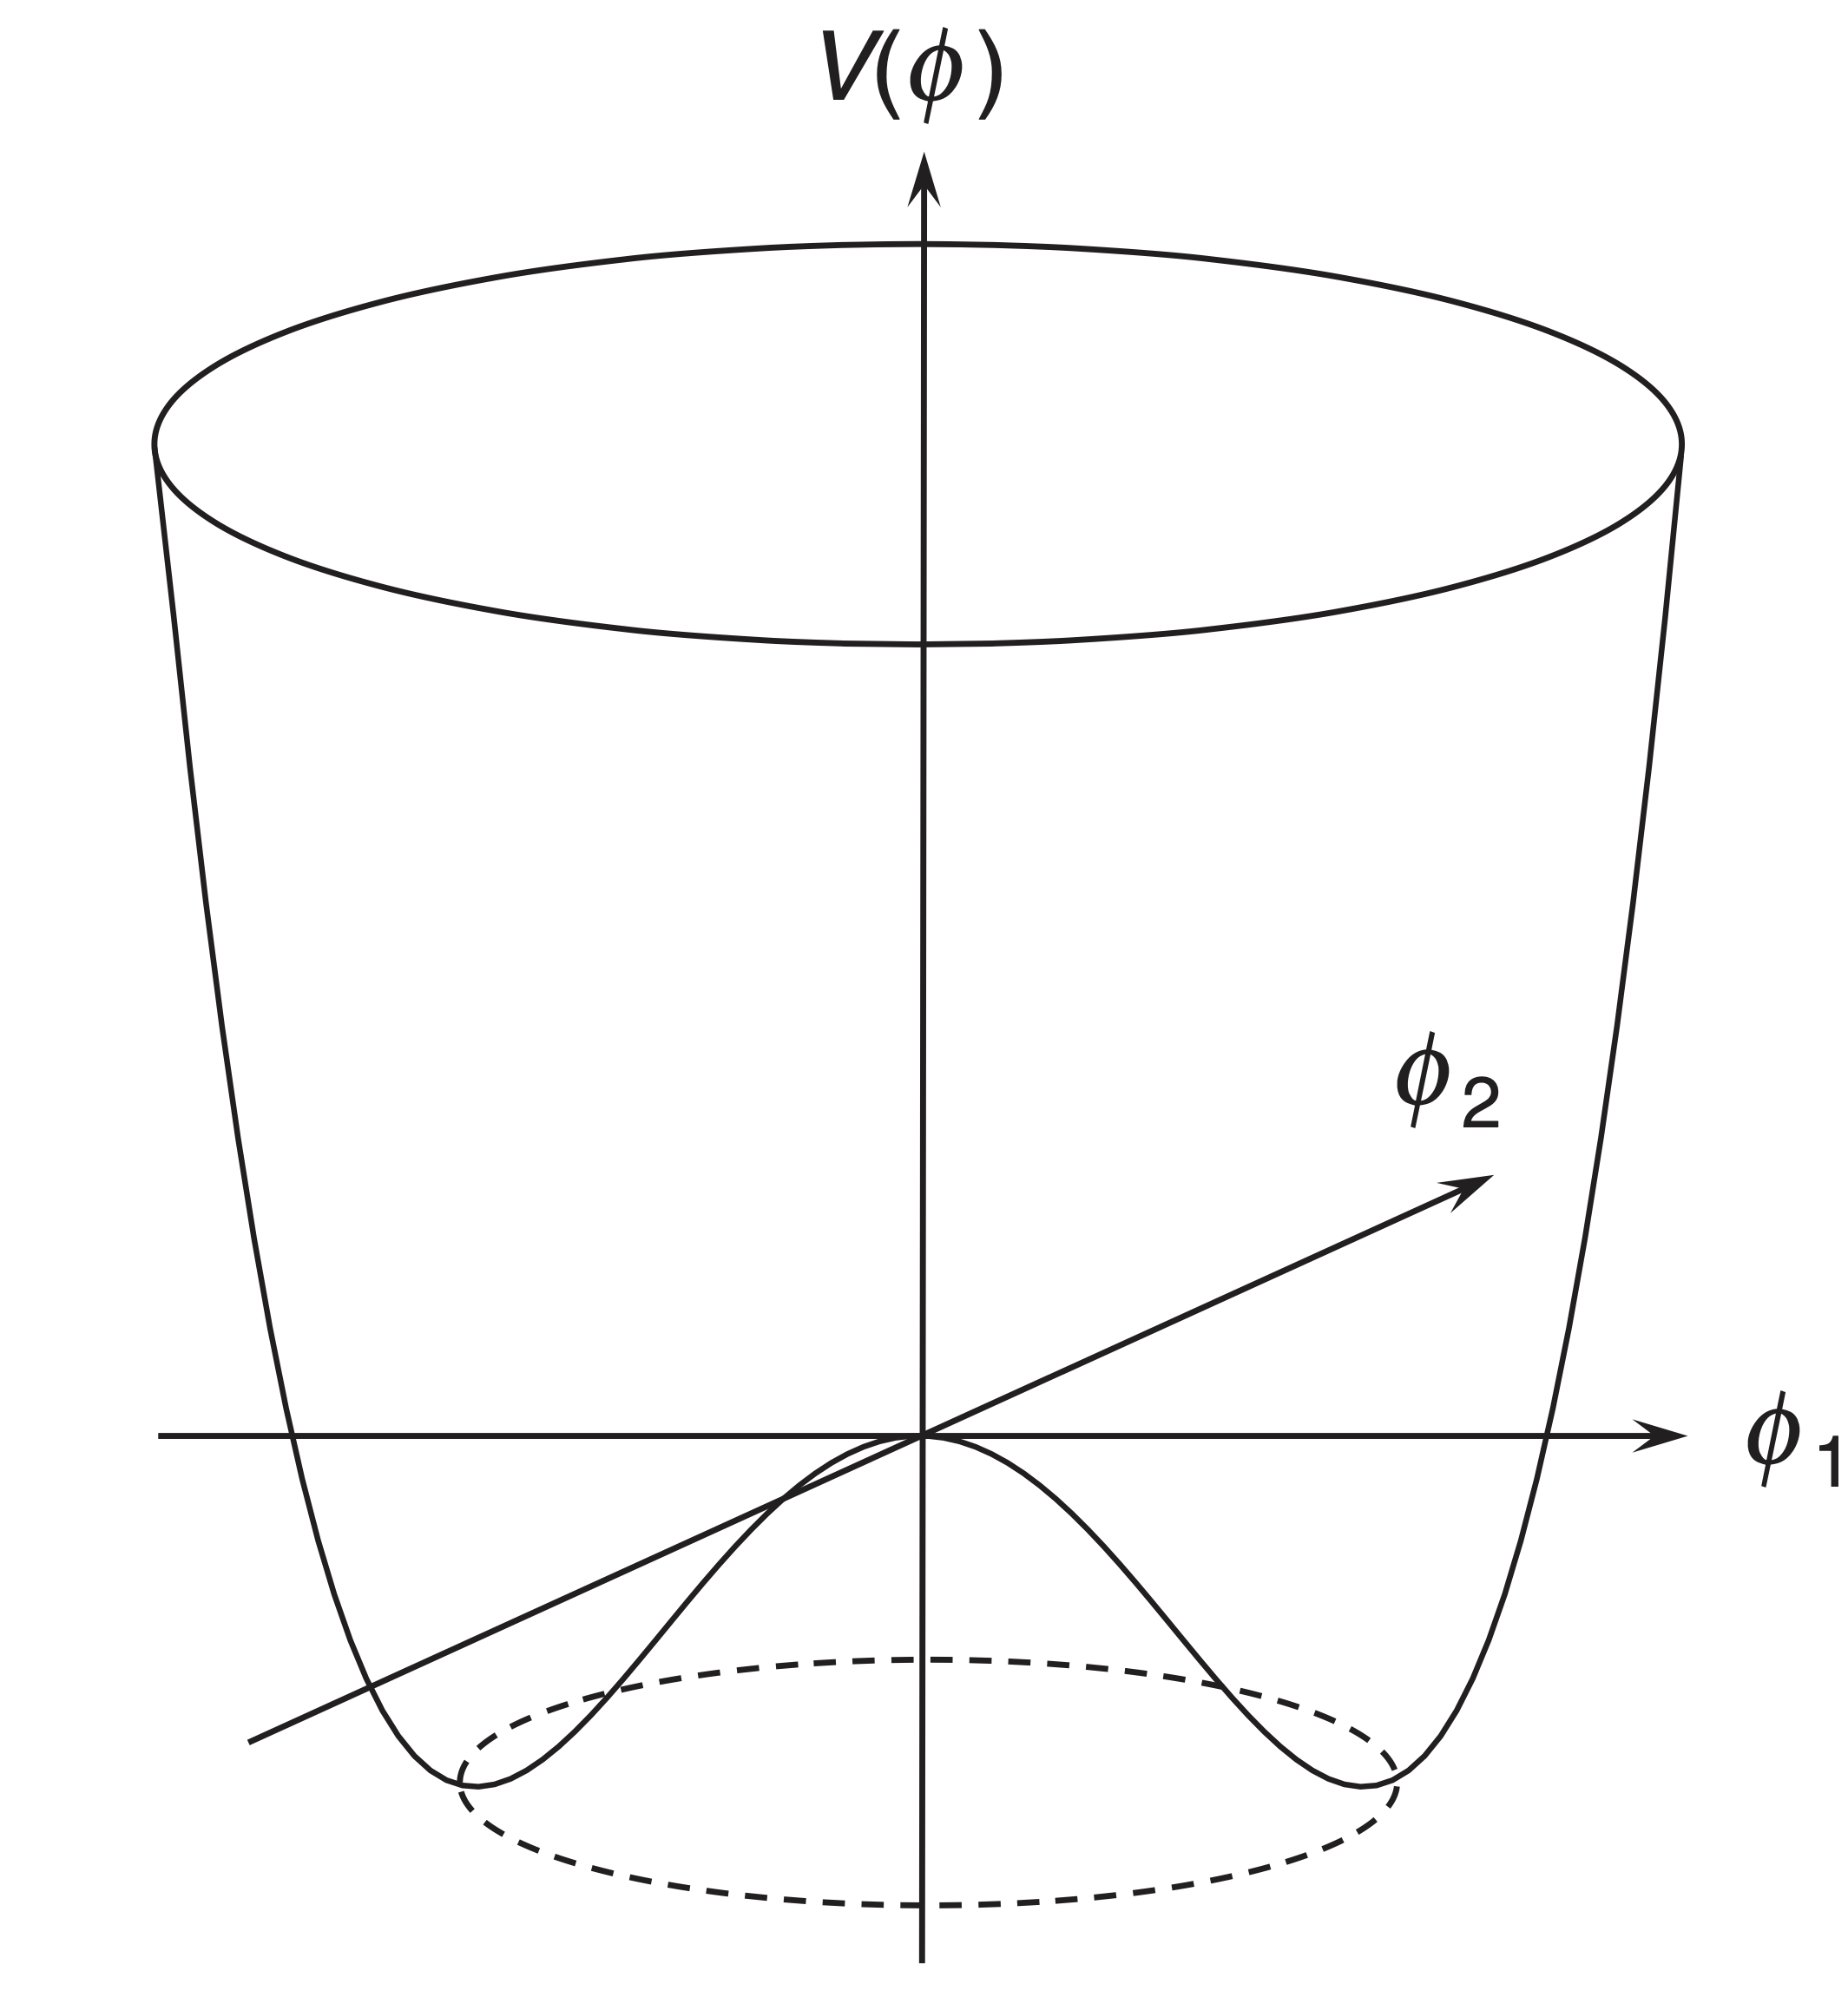
\includegraphics[width=.5\textwidth]{Images/Theory/HiggsPotential.png}}
    \caption{A graph of the Higgs potential $V(\phi)$ as a function of the complex scalar Higgs field $\phi$ with real and imaginary components $\phi_1$ and $\phi_2$.}
    \label{fig:HiggsPotential}
\end{figure}
